\documentclass[border=4pt]{standalone}
\usepackage{amsmath, amssymb, amsfonts}
\usepackage{tikz}
% Shared TikZ style for the deep-learning computation-graph figures.
% Change notation/appearance in ONE place here and rebuild all figures.
\usetikzlibrary{arrows.meta, positioning, calc}

% Colours for forward-pass / backprop highlights
\definecolor{fwdblue}{RGB}{0,0,255}
\definecolor{bpred}{RGB}{255,0,0}

\tikzset{
    % filled dot used for inputs, biases and indicator vectors
    unit/.style={circle, fill=black, inner sep=0pt, minimum size=5pt},
    % linear transformation node (weighted sum), drawn as a circled plus
    sumop/.style={circle, draw, thick, inner sep=1pt, minimum size=16pt},
    % non-linear transformation, a labelled box with vertical text
    opbox/.style={draw, thick, minimum width=22pt, inner sep=6pt},
    % directed edges
    edge/.style={-{Latex[length=6pt]}, thick},
    % edge labels (variable names on the wires)
    wire/.style={font=\normalsize, inner sep=2pt},
}

% vertical text for the operation boxes
\newcommand{\vlabel}[1]{\rotatebox{90}{#1}}


\begin{document}
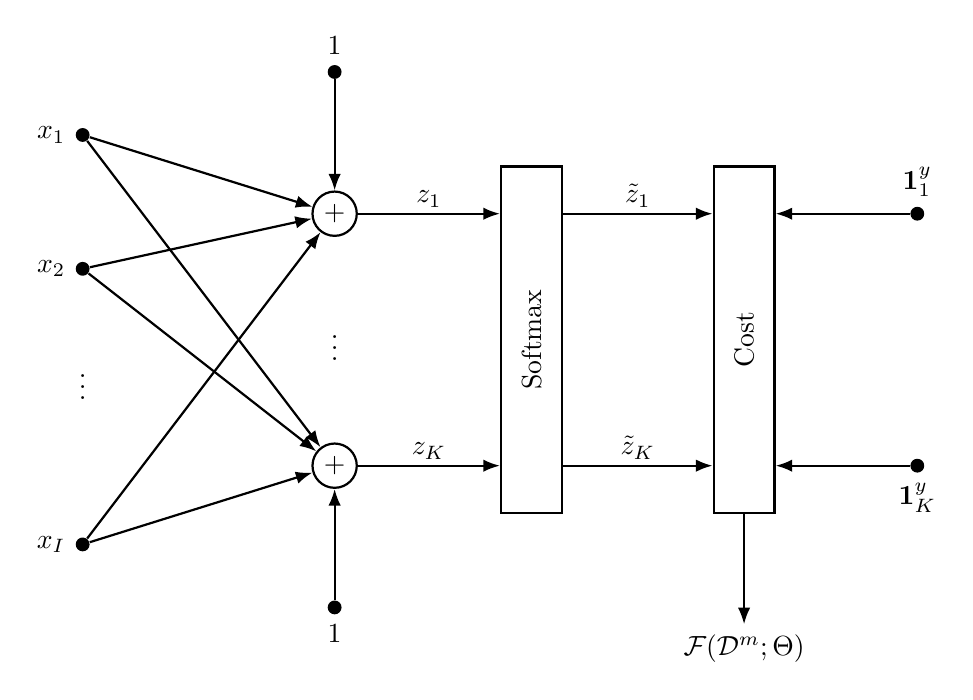
\begin{tikzpicture}[>=Latex]

    % --- linear (sum) nodes ---
    \node[sumop] (sA) at (3.2, 1.6)  {$+$};
    \node[sumop] (sB) at (3.2, -1.6) {$+$};
    \node at (3.2, 0) {$\vdots$};

    % --- inputs ---
    \node[unit, label=left:{$x_1$}] (x1) at (0, 2.6)  {};
    \node[unit, label=left:{$x_2$}] (x2) at (0, 0.9)  {};
    \node                            (xd) at (0, -0.5) {$\vdots$};
    \node[unit, label=left:{$x_I$}] (xI) at (0, -2.6) {};

    % --- biases ---
    \node[unit, label=above:{$1$}] (bA) at (3.2, 3.4)  {};
    \node[unit, label=below:{$1$}] (bB) at (3.2, -3.4) {};

    % fully-connected input -> sum edges
    \foreach \x in {x1,x2,xI}{
        \draw[edge] (\x) -- (sA);
        \draw[edge] (\x) -- (sB);
    }
    \draw[edge] (bA) -- (sA);
    \draw[edge] (bB) -- (sB);

    % --- non-linear boxes ---
    \node[opbox, minimum height=4.4cm] (soft) at (5.7, 0) {\vlabel{Softmax}};
    \node[opbox, minimum height=4.4cm] (cost) at (8.4, 0) {\vlabel{Cost}};

    % sum -> softmax (z)
    \draw[edge] (sA) -- (soft.west |- sA) node[wire, midway, above] {$z_1$};
    \draw[edge] (sB) -- (soft.west |- sB) node[wire, midway, above] {$z_K$};

    % softmax -> cost (tilde z)
    \draw[edge] (soft.east |- sA) -- (cost.west |- sA)
        node[wire, midway, above] {$\tilde{z}_1$};
    \draw[edge] (soft.east |- sB) -- (cost.west |- sB)
        node[wire, midway, above] {$\tilde{z}_K$};

    % indicator inputs on the right, pointing into Cost
    \node[unit, label=above:{$\mathbf{1}^y_1$}] (i1) at (10.6, 1.6)  {};
    \node[unit, label=below:{$\mathbf{1}^y_K$}] (iK) at (10.6, -1.6) {};
    \draw[edge] (i1) -- (cost.east |- sA);
    \draw[edge] (iK) -- (cost.east |- sB);

    % cost output
    \draw[edge] (cost.south) -- ++(0, -1.4)
        node[below] {$\mathcal{F}(\mathcal{D}^m; \Theta)$};

\end{tikzpicture}
\end{document}
